\chapter{look back time}

Agarre el Void S mas alla de el radio de void (15 < r > 25) donde la densidad es mas parecida que a la del universo  e hice los diagramas de fase a diferentes redshift. 

\begin{figure}[h]
\centering
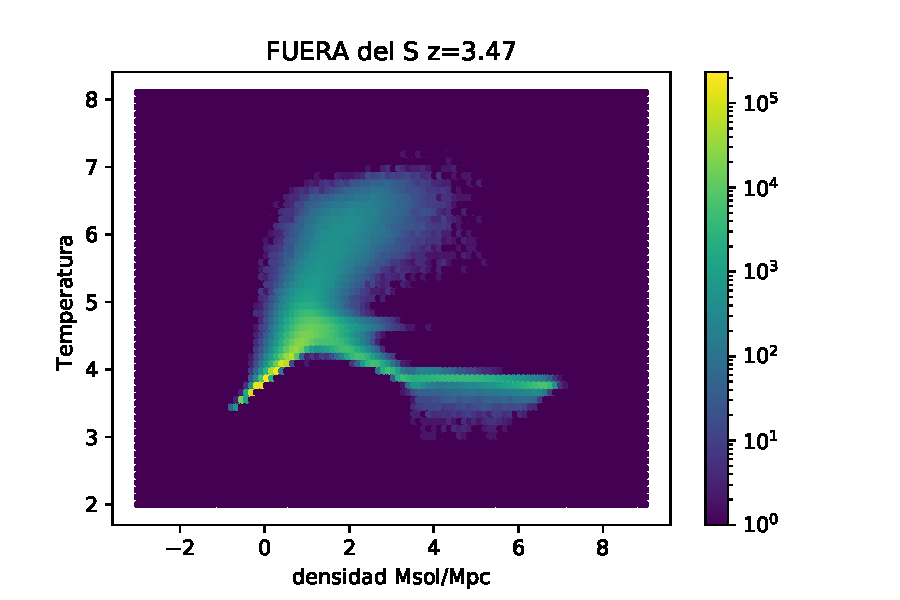
\includegraphics[width=18cm]{Figures/S_df_s25.pdf}
\decoRule
\caption[Fraccione stellar vs gas]{Fracciones de gs/dm vs estrellas/dm }
\label{fig:Electron}
\end{figure}

\begin{figure}[h]
\centering
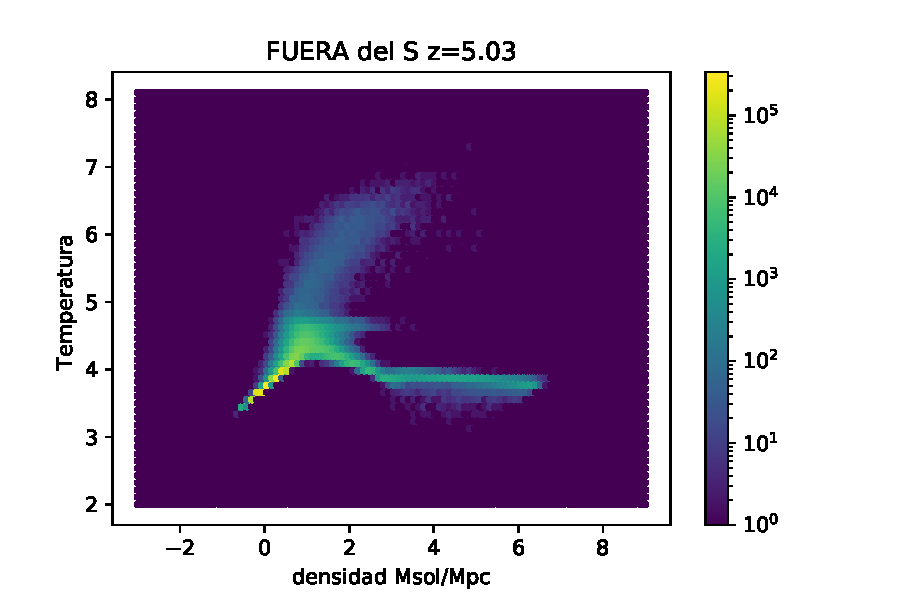
\includegraphics[width=18cm]{Figures/S_df_s20.pdf}
\decoRule
\caption[Fraccione stellar vs gas]{Fracciones de gs/dm vs estrellas/dm }
\label{fig:Electron}
\end{figure}

\begin{figure}[h]
\centering
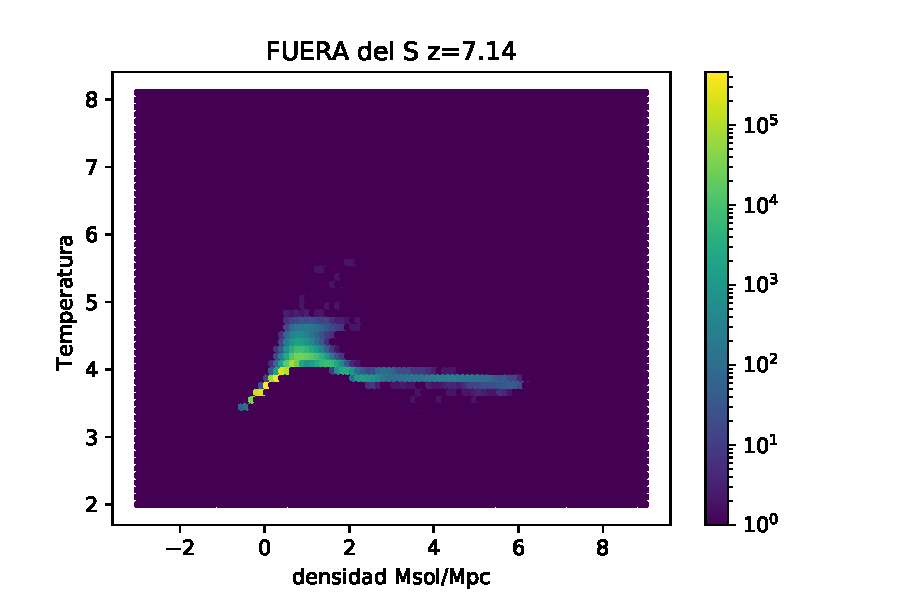
\includegraphics[width=18cm]{Figures/S_df_s15.pdf}
\decoRule
\caption[Fraccione stellar vs gas]{Fracciones de gs/dm vs estrellas/dm }
\label{fig:Electron}
\end{figure}